\subsubsection{usergoal-ugCrisisInTime}

\label{RE-use-case-ugCrisisInTime}


An actor has been login as a Administrator to use the statistic function. So he can see the number of crises compared with the time		  


\begin{usecase}
  \addheading{Use-Case Description}
  \addsingletwocolumnrow{Name}{ugCrisisInTime}
  \addsingletwocolumnrow{Scope}{system}
  \addsingletwocolumnrow{Level}{usergoal}
  

\addrowheading{Primary actor(s)}
\addnumberedsinglerow{}{\msrcode{actAdministrator[active]}}
\addnumberedsinglerow{}{\msrcode{actDatabase[proactive]}}


\addrowheading{Secondary actor(s)}
\addnumberedsinglerow{}{\msrcode{actSystem[active]}}

\addrowheading{Goal(s) description}
\addsinglerow{An actor has been login as a Administrator to use the statistic function. So he can see the number of crises compared with the time}

\addrowheading{Reuse}
\addnumberedsinglerow{}{\msrucname{oeStatistic [1..*]}}
\addnumberedsinglerow{}{\msrucname{ugSercurelyUserSystem [0..*]}}
\addnumberedsinglerow{}{\msrucname{oeNumberOfCrisis [0..*]}}
\addnumberedsinglerow{}{\msrucname{ugAdministrateTheSystem [1..*]}}

\addrowheading{Protocol condition(s)}
\addnumberedsinglerow{}{The actor  has been login as a administrator and he has to click on the button static.
}
\addnumberedsinglerow{}{The actor must be able to access the system (connected to the internet)}

\addrowheading{Pre-condition(s)}
\addnumberedsinglerow{}{The actor is not login as a administrator, so he can click the button statistic.
}

\addrowheading{Main post-condition(s)}
\addnumberedsinglerow{}{if the login was successful, the actor is now identified and thus able to access the AdministrateTheSystem
}
\addnumberedsinglerow{}{The actor can click the button statistic and so he see the statistic
}

\addrowheading{Main Steps}
\addalphanumberedsinglerow{}{the actor \msrcode{actSystem} executes the \msrucname{ugSercurelyUserSystem} use case}
\addalphanumberedsinglerow{}{the actor \msrcode{actSystem} executes the \msrucname{oeStatistic} use case}
\addalphanumberedsinglerow{}{the actor \msrcode{actAdministrator} executes the \msrucname{oeNumberOfCrisis} use case}
\addalphanumberedsinglerow{}{the actor \msrcode{actAdministrator} executes the \msrucname{ugAdministrateTheSystem} use case}
\addalphanumberedsinglerow{}{the actor \msrcode{actDatabase} executes the \msrucname{oeNumberOfCrisis} use case}
\addrowheading{Steps Ordering Constraints}
\addnumberedsinglerow{}{at least a}
\addnumberedsinglerow{}{if b then previously a}
\addnumberedsinglerow{}{if c then previously b}
\addnumberedsinglerow{}{if d then previously c}

\addrowheading{Additional Information}
\addsinglerow{
none
}

\end{usecase} 


Figure \ref{fig:lu.uni.lassy.excalibur.examples.icrash-RE-UCD-uc-ugCrisisInTime}
The actor administrator will open the statics The number of crisis at the time, there he can find out how many crisis are send at the different time. Also the abstract user System give the information 

\begin{figure}[htbp]
\begin{center}

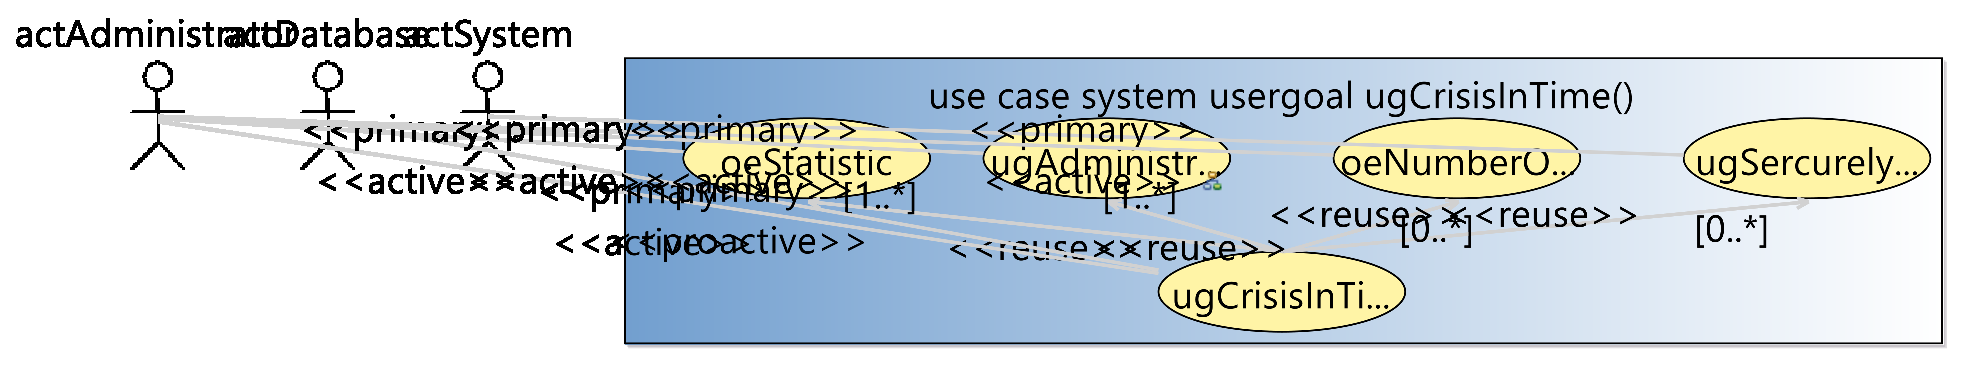
\includegraphics[
angle=0
,width=1.0\textwidth
]{./images-report-gen/usecase-model/usergoal/uc-ugCrisisInTime.eps}
\end{center}
\caption[lu.uni.lassy.excalibur.examples.icrash Use Case Diagram: uc-ugCrisisInTime]{The number of crisis at the time}
\label{fig:lu.uni.lassy.excalibur.examples.icrash-RE-UCD-uc-ugCrisisInTime}
\end{figure}
\vspace{0.5cm}
